\documentclass{beamer}

% Theme selection
\usetheme{Madrid}
\usefonttheme{serif}
\usecolortheme{beaver}

% Packages
\usepackage{booktabs}
\usepackage{graphicx}
\usepackage{amsmath}
\usepackage{algorithm}
\usepackage{algpseudocode}

% Title Info
\title{Lab 1: Decision Trees}
\subtitle{DD2421 Machine Learning}
\author{Lucas Frykman}
\date{\today}

\begin{document}

% Title Slide
\begin{frame}
    \titlepage
\end{frame}

% Assignment 0
\begin{frame}{Assignment 0: Dataset Difficulty}
    \textbf{Question:} Which dataset is the most difficult to learn? \\
    \textbf{Monk-1}: $(a_1=a_2)\lor(a_5=1)$ \\
    This set is the easiest. Only 3 attributes are needed to be known to predict (i.e optimal
    tree depth is 3).
    \\ \textbf{Monk-2}: $a_i$ for exactly 2 $i$ \\
    Decision trees struggle with this because the information 
    is not contained in individual attribute splits.
    Each attribute by itself contains zero information. 
    We need to know all 5 attributes simultaenously to classify a sample (i.e tree depth is 5).
    \\ \textbf{Monk-3} $(a_5=1\land a_4=1)\lor(a_5 \neq 4 \land a_4 \neq 3)$ \\
    This set is the second hardest. It has 5\% noise which will lead to bad generalization. But it won't need much more than a depth of 3.

\end{frame}

% Assignment 1 & 2
\begin{frame}{Assignment 1 \& 2: Entropy}
    \textbf{Assignment 1: Dataset Entropy}
    \begin{itemize}
        \item Monk-1: 1.0
        \item Monk-2: 0.957
        \item Monk-3: 0.999
    \end{itemize}

    \vspace{1em}
    \textbf{Assignment 2: Understanding Entropy}
    \begin{itemize}
        \item \textbf{Definition:} Entropy quantifies the uncertainty in a distribution.
        \item \textbf{Uniform Distribution (Max Entropy):} All outcomes are equally likely and is hardest to predict. Example: A fair coin
        \item \textbf{Skewed Distribution (Low Entropy):} One outcome dominates and is easier to predict. Example: Height measurement
    \end{itemize}
\end{frame}

% Assignment 3
\begin{frame}{Assignment 3: Information Gain}
    \textbf{Selecting the root node:} We select the attribute with the highest Information Gain (IG).

    \begin{table}[]
        \centering
        \resizebox{\textwidth}{!}{%
        \begin{tabular}{lcccccc}
        \toprule
        \textbf{Dataset} & \textbf{A1} & \textbf{A2} & \textbf{A3} & \textbf{A4} & \textbf{A5} & \textbf{A6} \\
        \midrule
        Monk-1 & 0.075 & 0.006 & 0.005 & 0.026 & \textbf{0.287} & 0.001 \\
        Monk-2 & 0.004 & 0.001 & 0.001 & 0.016 & \textbf{0.017} & 0.006 \\
        Monk-3 & 0.007 & \textbf{0.294} & 0.001 & 0.003 & 0.256 & 0.007 \\
        \bottomrule
        \end{tabular}%
        }
    \end{table}
    
    \begin{itemize}
        \item \textbf{Monk-1:} Split on A5.
        \item \textbf{Monk-2:} Split on A5.
        \item \textbf{Monk-3:} Split on A2.
    \end{itemize}
\end{frame}

% Assignment 4
\begin{frame}{Assignment 4: Motivation for Information Gain}
    \textbf{Why maximize Information Gain?} \\
    $\operatorname{Gain}(S,A) = H[S] - \sum_{v \in \operatorname{value}(A)} \frac{S_{A=v}}{S}H[S|A=v] = H[S] - E[H[S|A]]$ \\ 
    \begin{itemize}
        \item \textbf{Reducing Impurity:} Maximizing IG is mathematically equivalent to minimizing the expected entropy 
            of a attribute A. We choose this as the root then repeat for its children.
            We want subsets that are as pure as possible
        \item \textbf{Heuristic Efficiency:} By choosing the attribute that best separates the classes early on, we create a shallower, simpler tree.
        \item \textbf{Generalization:} Simpler trees tend to generalize better to unseen data compared to unnecessarily deep trees
    \end{itemize}
\end{frame}

% Assignment 5
\begin{frame}{Assignment 5: Full Tree Performance}
    We built full decision trees using ID3 and evaluated them on the test sets.

    \begin{table}[]
        \centering
        \begin{tabular}{lcc}
        \toprule
        \textbf{Dataset} & \textbf{$E_{train}$} & \textbf{$E_{test}$} \\
        \midrule
        Monk-1 & 0.0 & 0.1713 \\
        Monk-2 & 0.0 & 0.3079 \\
        Monk-3 & 0.0 & 0.0556 \\
        \bottomrule
        \end{tabular}
    \end{table}
    
    \textbf{Observations:}
    \begin{itemize}
        \item $E_{train}$ is 0 for all, indicating the trees fully memorized the training data (overfitting).
        \item Monk-2 has the highest test error, confirming it is the hardest concept to learn using standard splits
    \end{itemize}
\end{frame}

% Assignment 6
\begin{frame}{Assignment 6: Pruning \& Bias-Variance}
    \textbf{The Bias-Variance Trade-off} \\
    \begin{itemize}
        \item \textbf{Full Trees (High Variance):} They fit the training data perfectly (low bias) but capture noise, 
            leading to poor generalization (high variance).
        \item \textbf{Pruning (Reducing Variance):} By removing branches that don't provide much information, we simplify the model.
        \item Pruning slightly increases bias (we might miss some training nuances) but significantly decreases variance so the model becomes less sensitive to to the training data set.
            leading to a lower total error on the test set
    \end{itemize}
\end{frame}


\begin{frame}{Assignment 7: Pruning Analysis}
\begin{algorithmic}[1]
\Function{PruneTree}{$T$, $V$}
    \State $T_{current} \gets T$
    \State $bestAcc \gets \textsc{Accuracy}(T_{current}, V)$
    \While{true}
        \State $Candidates \gets \textsc{AllPruned}(T_{current})$
        \If{$Candidates$ is empty}
            \State \Return $T_{current}$
        \EndIf
        \State $T_{best} \gets 
        \displaystyle\arg\max_{T' \in Candidates}
        \textsc{Accuracy}(T', V)$
        \State $candidateAcc \gets 
        \textsc{Accuracy}(T_{best}, V)$
        \If{$candidateAcc \geq bestAcc$}
            \State $T_{current} \gets T_{best}$
            \State $bestAcc \gets candidateAcc$
        \Else
            \State \Return $T_{current}$
        \EndIf
    \EndWhile
\EndFunction
\end{algorithmic}
\end{frame}
% Assignment 7
\begin{frame}{Assignment 7: Pruning Analysis}
    We performed Reduced Error Pruning with different training/validation splits ($N=5000$ iterations where the split was shuffled). 
    
    \begin{itemize}
        \item \textbf{Monk-1:} Optimal performance around split 60:40 but has slightly higher variance. Less biased for less training data. 
        \item \textbf{Monk-3:} Optimal performance around split 70:30 and slightly lower variance. Higher variance for less training data due
            to noise 
    \end{itemize}

    \begin{figure}
        \centering
        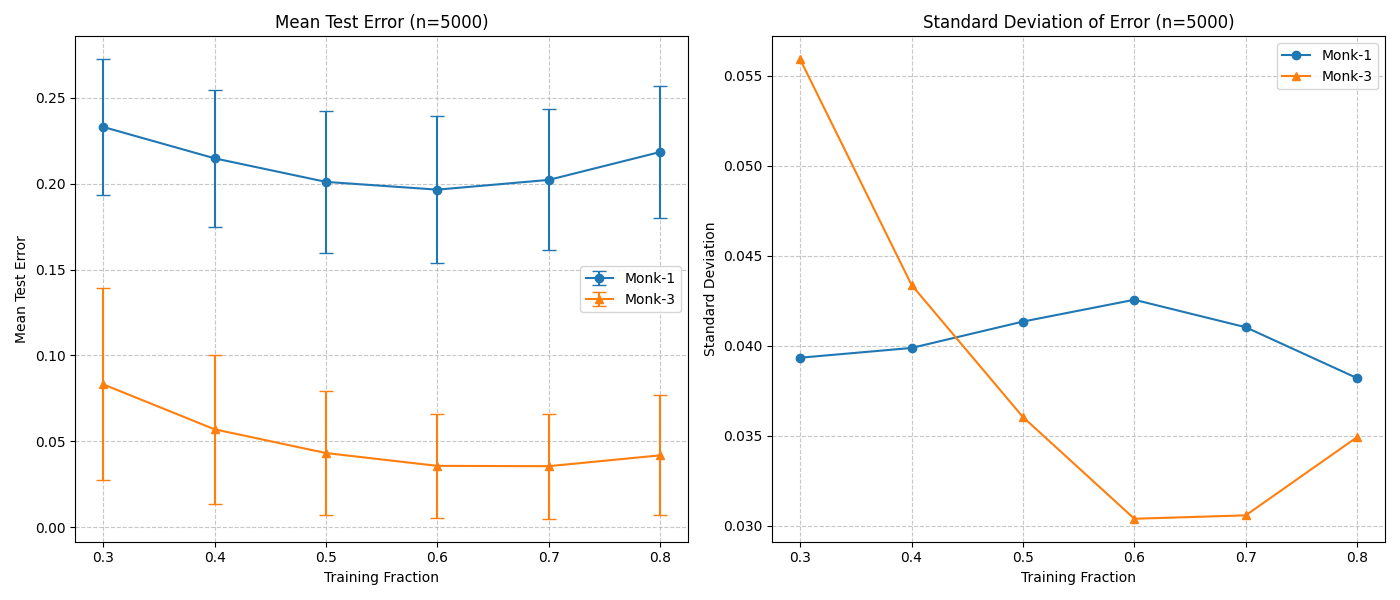
\includegraphics[width=0.7\textwidth]{image1.png}
        \caption{Mean test error vs. Training Fraction}
    \end{figure}
\end{frame}

\begin{frame}{Assignment 7: Pruning Analysis}
    Monk 1
    \centering
    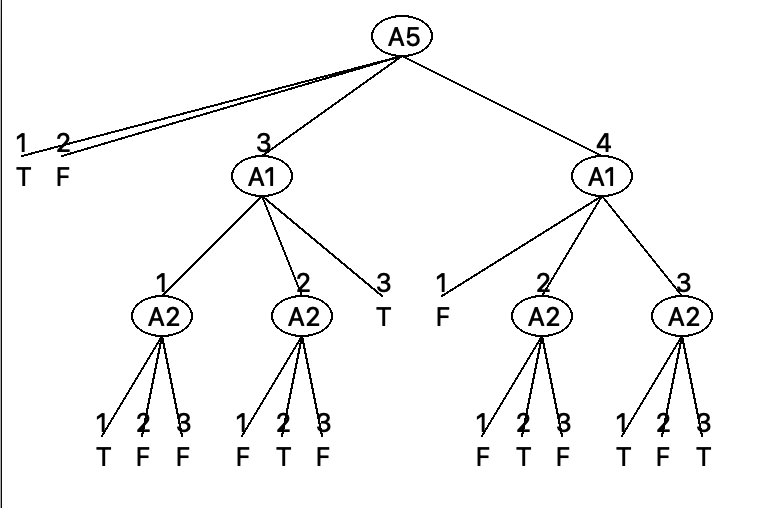
\includegraphics[width = 0.7\textwidth]{pruned_monk1}
\end{frame}
\begin{frame}{Assignment 7: Pruning Analysis}
    Monk 3
    \centering
    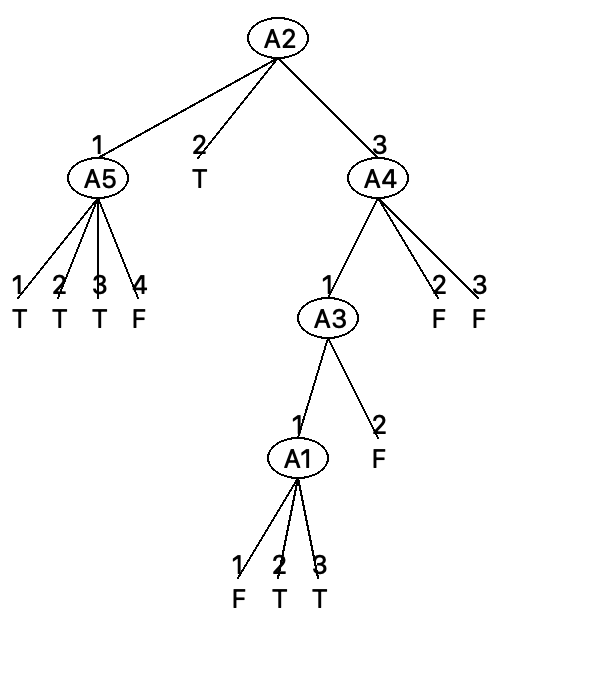
\includegraphics[width = 0.6\textwidth]{pruned_monk2}
\end{frame}
\end{document}
